\documentclass[11pt, oneside]{article}   	% use "amsart" instead of "article" for AMSLaTeX format
\usepackage[margin=1in]{geometry}                		% See geometry.pdf to learn the layout options. There are lots.
\geometry{letterpaper}                   		% ... or a4paper or a5paper or ... 
%\geometry{landscape}                		% Activate for rotated page geometry
%\usepackage[parfill]{parskip}    		% Activate to begin paragraphs with an empty line rather than an indent
\usepackage{graphicx}				% Use pdf, png, jpg, or eps§ with pdflatex; use eps in DVI mode
								% TeX will automatically convert eps --> pdf in pdflatex		
\usepackage{amssymb}
\usepackage{awesomebox}
%SetFonts

%SetFonts

\usepackage{amsmath}
\DeclareMathOperator{\plainmod}{\text{ mod }}
\let\emptyset\varnothing

\newcommand{\reals}{\mathbb{R}}
\newcommand{\realsText}{$\mathbb{R}$}
\newcommand{\ints}{\mathbb{Z}}
\newcommand{\intsText}{$\mathbb{Z}$}

\title{Homework 5}
\author{Discrete Structures 2}
\date{due: 13 April 2023, 8:00am}							% Activate to display a given date or no date

\begin{document}
\maketitle
%\section{}
%\subsection{}

Your task for this homework will be to answer the following questions without using any calculating resources. 
Your responses should be submitted via blackboard by the due date above as a PDF (submissions in any other format will be returned to the user and a resubmissions will be requested). 
You are free to use whatever tools you would like to generate the response document: 
scanned hand-written paper, 
tablet generated hand-written, 
microsoft word (with this option, please use the equation editor to correctly format your responses), 
\LaTeX, etc.
Your TA, IA, and Instructor are available to help during their designated office hours or via email 
(note that emails sent during non-business hours may not be responded to until the next working day). 

%\importantbox{
%\textbf{Note:} all of these questions are on topics from chapters 5; thus you will only be proving by induction in this homework assignment. 
%}
\begin{enumerate}
%9.124-129
 \item
For two strings x and y, let’s call a shuffle of x and y any interleaving of the letters of the two strings (that maintains the order of the letters within each string, but may repeatedly alternate between blocks of x letters and blocks of y letters). For example, the words \texttt{ALE} and \texttt{LID} can be shuffled into\\
\begin{center} 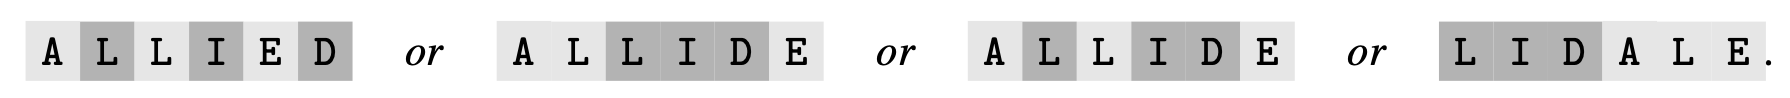
\includegraphics[width=.9\textwidth]{HW5_shuffle} \end{center}
 How many different strings can be produced as shuffles of the following pairs of words?
\begin{enumerate}
\item \texttt{BACK} and \texttt{FORTH}
\item \texttt{DAY} and \texttt{NIGHT}
\item \texttt{SUPPLY} and \texttt{DEMAND}
\item \texttt{LIFE} and \texttt{DEATH}
\item \texttt{ON} and \texttt{ON}
\item \texttt{OUT} and \texttt{OUT}
\end{enumerate}

%9.138
\item What is the smallest even integer $n$ for which the following statement is true?
If we flip an unbiased coin $n$ times, as in the example from class,
the probability that we get exactly $\frac{n}{2}$ heads is less than $10\%$.

%9.148-151
\item 
How many ways are there to choose $32$ out of $202$ options if 
\begin{enumerate}
\item repetition is allowed and order matters?
\item repetition is forbidden and order matters?
\item repetition is allowed and order doesn't matter?
\item repetition is forbidden and order doesn't matter?
\end{enumerate}

%9.160
\item Consider the equation $a+b+c=202$. How many solutions are there where $a,b,$ and $c$ are all nonnegative integers?
%9.161 
\item How many solutions are there to the equation $a+b+c+d+e=8$, where all of $\{a,b,c,d,e\}$ must be nonnegative integers?
%9.162 
\item What about for $a+b+c+d+e=88$, again where all variables must be nonnegative integers?
%9.163 
\item What about for $a+2b+c=128$, again where $a,b,$ and $c$ must be nonnegative integers? (Hint: sum over the possible values of $b$ and use the slide ``Choosing with repetition when order doesn’t matter'' from the slides/Theorem 9.16 in the book.)


\end{enumerate}
\end{document}